\chapter{Specifikacija programske potpore}
		
	\section{Funkcionalni zahtjevi}
			
			\textbf{\textit{dio 1. revizije}}\\
			
			\textit{Navesti \textbf{dionike} koji imaju \textbf{interes u ovom sustavu} ili  \textbf{su nositelji odgovornosti}. To su prije svega korisnici, ali i administratori sustava, naručitelji, razvojni tim.}\\
				
			\textit{Navesti \textbf{aktore} koji izravno \textbf{koriste} ili \textbf{komuniciraju sa sustavom}. Oni mogu imati inicijatorsku ulogu, tj. započinju određene procese u sustavu ili samo sudioničku ulogu, tj. obavljaju određeni posao. Za svakog aktora navesti funkcionalne zahtjeve koji se na njega odnose.}\\
			
			
			\noindent \textbf{Dionici:}
			
			\begin{packed_enum}
				
				\item Vlasnik kućnog ljubimca
				\item Sklonište za životinje			
				\item Ostali korisinici aplikacije(klijent?)
                \item Razvojni tim
				
			\end{packed_enum}
			
			\noindent \textbf{Aktori i njihovi funkcionalni zahtjevi:}
			
			
			\begin{packed_enum}
				\item  \underbar{Neregistrirani korisnik (inicijator) može:}
				
				\begin{packed_enum}
					
					\item funkcionalnost 1
					\item funkcionalnost 2
					\begin{packed_enum}
						
						\item  podfunkcionalnost 1 
						\item  podfunkcionalnost 2
				
					\end{packed_enum}
					\item  funkcionalnost 3
					
				\end{packed_enum}

                \item  \underbar{Vlasnik kućnog ljubimca (inicijator) može:}
				
				\begin{packed_enum}
					
					\item funkcionalnost 1
					\item funkcionalnost 2
					
				\end{packed_enum}

                \item  \underbar{Skloništa za životinje (inicijator) može:}
				
				\begin{packed_enum}
					
					\item funkcionalnost 1
					\item funkcionalnost 2
					
				\end{packed_enum}
			
				\item  \underbar{Baza podataka (sudionik) može:}
				
				\begin{packed_enum}
					
					\item funkcionalnost 1
					\item funkcionalnost 2
					
				\end{packed_enum}
			\end{packed_enum}
			
			\eject 
			
			
				
			\subsection{Obrasci uporabe}
				
				\textbf{\textit{dio 1. revizije}}
				
				\subsubsection{Opis obrazaca uporabe}		

					\noindent \underbar{\textbf{UC1 - Pregled nestalih ljubimaca}}
					\begin{packed_item}
	
						\item \textbf{Glavni sudionik: }Korisnik, Registrirani korisnik, Sklonište
						\item  \textbf{Cilj:} Pregledavanje oglašenih nestalih kućnih ljubimaca i skloništa za životinje
						\item  \textbf{Sudionici:} Baza podataka
						\item  \textbf{Preduvjet:} -
						\item  \textbf{Opis osnovnog tijeka:}
						
						\item[] \begin{packed_enum}
	
							\item Nestali ljubimci su prikazani prilikom učitavanja aplikacije
							\item Korisnik odabire nestalog ljubimca
							\item Prikazuje se detaljniji pregled informacija i pregled komunikacija oko potrage
						\end{packed_enum}
						
					\end{packed_item}
				
					\noindent \underbar{\textbf{UC2 - Registracija}}
					\begin{packed_item}
						
						\item \textbf{Glavni sudionik: }Korisnik 
						\item  \textbf{Cilj:} Stvoriti korisnički račun za pristup sustavu
						\item  \textbf{Sudionici:} Baza podataka
						\item  \textbf{Preduvjet:} -
						\item  \textbf{Opis osnovnog tijeka:}
						
						\item[] \begin{packed_enum}
							
							\item Korisnik odabire opciju za registraciju
							\item Korisnik unosi vlastite podatke
							\item Podaci se spremaju u bazu podataka
							\item Korisnik prima obavijest o uspješnoj registraciji
						\end{packed_enum}
						
						\item  \textbf{Opis mogućih odstupanja:}
						
						\item[] \begin{packed_item}
							
							\item[2.a] Podaci koje je korisnik unio odgovaraju postojećem korisničkom računu
							\item[] \begin{packed_enum}
								
								\item Pojavljuje se poruka o neuspješnoj registraciji i zahtjev za ponovnim unosom podataka
								\item Korisnik mijenja podatke ili odustaje od registracije
								
							\end{packed_enum}
							\item[2.b] Korisnik nije unio sve zahtijevane podatke
								\item[] \begin{packed_enum}
								
								\item Pojavljuje se poruka o neuspješnoj registraciji i zahtjev za ponovnim unosom podataka
								\item Korisnik unosi zahtijevane podatke ili odustaje od registracije
								
							\end{packed_enum}
							
						\end{packed_item}
					\end{packed_item}
					
					\noindent \underbar{\textbf{UC3 - Pretraživanje nestalih ljubimaca}}
					\begin{packed_item}
						
						\item \textbf{Glavni sudionik: }Korisnik, Registrirani korisnik, Sklonište
						\item  \textbf{Cilj:} Pretraživanje nestalih ljubimaca po svim dostupnim kategorijama podataka
						\item  \textbf{Sudionici:} Baza podataka
						\item  \textbf{Preduvjet:} -
						\item  \textbf{Opis osnovnog tijeka:}
						
						\item[] \begin{packed_enum}
							
							\item Korisnik odabire kategorije podataka po kojima obavlja pretraživanje
							\item Korisnik unosi podatke (filtre) za odabrane kategorije
							\item Prikazuje se popis filtriranih oglasa
						\end{packed_enum}
					\end{packed_item}
					
					\noindent \underbar{\textbf{UC4 - Prijava u sustav}}
					\begin{packed_item}
						
						\item \textbf{Glavni sudionik: }Registrirani korisnik, Sklonište
						\item  \textbf{Cilj:} Dobiti pristup korisničkom sučelju
						\item  \textbf{Sudionici:} Baza podataka
						\item  \textbf{Preduvjet:} Registracija
						\item  \textbf{Opis osnovnog tijeka:}
						
						\item[] \begin{packed_enum}
							
							\item Unos korisničkog imena ili e-mail adrese i lozinke
							\item Provjera ispravnosti unesenih podataka
							\item Pristup korisničkom sučelju web aplikacije
						\end{packed_enum}
						
						\item  \textbf{Opis mogućih odstupanja:}
						
						\item[] \begin{packed_item}
							
							\item[2.a] Korisnik je unio nepostojeće korisničko ime ili e-mail adresu
							\item[] \begin{packed_enum}
								
								\item Pojavljuje se poruka o neuspješnoj prijavi i zahtjev za ponovnim unosom podataka
								\item Korisnik unosi ispravne podatke ili odustaje od prijave
								
							\end{packed_enum}
							\item[2.b] Korisnik je unio neispravnu lozinku za odgovarajuće korisničko ime odnosno e-mail
							\item[] \begin{packed_enum}
								
								\item Pojavljuje se poruka o neuspješnoj prijavi i zahtjev za ponovnim unosom podataka
								\item Korisnik unosi ispravne podatke ili odustaje od prijave
								
							\end{packed_enum}
							
						\end{packed_item}
					\end{packed_item}
					\pagebreak
					\noindent \underbar{\textbf{UC5 - Komuniciranje oko potrage}}
					\begin{packed_item}
						
						\item \textbf{Glavni sudionik: }Registrirani korisnik, Sklonište
						\item  \textbf{Cilj:} Ostvariti komunikaciju s vlasnikom izgubljenog ljubimca
						\item  \textbf{Sudionici:} Baza podataka
						\item  \textbf{Preduvjet:} Korisnik je prijavljen
						\item  \textbf{Opis osnovnog tijeka:}
						
						\item[] \begin{packed_enum}
							
							\item Korisnik odabire nestalog ljubimca
							\item Prikazuje se popis komunikacije oko potrage za ljubimcem
							\item Korisnik unosi poruku koja može sadržavati tekst, sliku i geolokaciju
						\end{packed_enum}
					\end{packed_item}
					
					\noindent \underbar{\textbf{UC6.1 - Postavljanje oglasa}}
					\begin{packed_item}
						
						\item \textbf{Glavni sudionik: }Registrirani korisnik, Sklonište 
						\item  \textbf{Cilj:} Postaviti oglas o izgubljenom ljubimcu
						\item  \textbf{Sudionici:} Baza podataka
						\item  \textbf{Preduvjet:} Korisnik je prijavljen
						\item  \textbf{Opis osnovnog tijeka:}
						
						\item[] \begin{packed_enum}
							
							\item Korisnik odabire opciju za novi oglas
							\item Korisnik unosi podatke o ljubimcu za zadane kategorije
							\item Korisnik objavljuje oglas
						\end{packed_enum}
						
						\item  \textbf{Opis mogućih odstupanja:}
						
						\item[] \begin{packed_item}
							
							\item[2.a] Korisnik je unio invalidne podatke u određenu kategoriju
							\item[] \begin{packed_enum}
								
								\item Pojavljuje se poruka o pogrešci i zahtjev za ponovnim unosom podataka
								\item Korisnik unosi ispravne podatke ili odustaje od objave oglasa
								
							\end{packed_enum}
							\item[2.b] Korisnik nije unio potrebne podatke
							\item[] \begin{packed_enum}
								
								\item Pojavljuje se poruka o pogrešci i zahtjev za ponovnim unosom podataka
								\item Korisnik unosi zahtijevane podatke ili odustaje od objave oglasa
								
							\end{packed_enum}
						\end{packed_item}
					\end{packed_item}
					\pagebreak
					\noindent \underbar{\textbf{UC6.2 - Uklanjanje oglasa}}
					\begin{packed_item}
						
						\item \textbf{Glavni sudionik: }Registrirani korisnik, Sklonište
						\item  \textbf{Cilj:} Ukloniti oglas o izgubljenom ljubimcu
						\item  \textbf{Sudionici:} Baza podataka
						\item  \textbf{Preduvjet:} Korisnik je prijavljen i objavio je oglas
						\item  \textbf{Opis osnovnog tijeka:}
						
						\item[] \begin{packed_enum}
							
							\item Korisnik odabire opciju za brisanje oglasa
							\item Korisnik potvrđuje akciju brisanja
							\item Oglas i sva komunikacija vezana uz njega nestaju iz popisa vidljivih oglasa
							\item Oglas ostaje pohranjen u bazi podataka
						\end{packed_enum}
						
						\item  \textbf{Opis mogućih odstupanja:}
						
						\item[] \begin{packed_item}
							
							\item[2.a] Korisnik odustaje od brisanja oglasa
						\end{packed_item}
					\end{packed_item}
					
					\noindent \underbar{\textbf{UC6.3 - Izmjena oglasa}}
					\begin{packed_item}
						
						\item \textbf{Glavni sudionik: }Registrirani korisnik, Sklonište
						\item  \textbf{Cilj:} Izmjena oglasa o izgubljenom ljubimcu
						\item  \textbf{Sudionici:} Baza podataka
						\item  \textbf{Preduvjet:} Korisnik je prijavljen i objavio je oglas
						\item  \textbf{Opis osnovnog tijeka:}
						
						\item[] \begin{packed_enum}
							
							\item Korisnik odabire opciju za izmjenu oglasa
							\item 
								\begin{packed_item}
									\item[a$)$] Korisnik mijenja podatke po kategorijama oglasa
									\item[b$)$] Korisnik mijenja kategoriju oglasa 
								\end{packed_item}
							\item Korisnik sprema promjene
						\end{packed_enum}
						
						\item  \textbf{Opis mogućih odstupanja:}
						
						\item[] \begin{packed_item}
							
							\item[2.a] Korisnik je unio invalidne podatke u određenu kategoriju
							\item[] \begin{packed_enum}
								
								\item  Pojavljuje se poruka o pogrešci i zahtjev za ponovnim unosom
								\item Korisnik unosi ispravne podatke ili odustaje od izmjene oglasa
								
							\end{packed_enum}
							\item[2.b] Korisnik je promijenio kategoriju oglasa u kategoriju koja ne odgovara aktivnoj potrazi za ljubimcem
							\begin{packed_enum}
								
								\item Oglas se prebacuje u popis neaktivnih oglasa
								
							\end{packed_enum}
							
						\end{packed_item}
					\end{packed_item}
					\pagebreak
					\noindent \underbar{\textbf{UC7 - Oglašavanje pronađenih životinja}}
					\begin{packed_item}
						
						\item \textbf{Glavni sudionik: }Sklonište
						\item  \textbf{Cilj:} Oglašavanje pronađenih životinja koje se nalaze u prostoru skloništa
						\item  \textbf{Sudionici:} Baza podataka
						\item  \textbf{Preduvjet:} Korisnik je prijavljen
						\item  \textbf{Opis osnovnog tijeka:}
						
						\item[] \begin{packed_enum}
							
							\item Korisnik odabire opciju za novi oglas
							\item Korisnik unosi podatke o ljubimcu za zadane kategorije (uključujući i dodatnu kategoriju – u skloništu)
							\item Korisnik objavljuje oglas
						\end{packed_enum}
						
						\item  \textbf{Opis mogućih odstupanja:}
						
						\item[] \begin{packed_item}
							
							\item[2.a] Korisnik je unio invalidne podatke u određenu kategoriju
							\item[] \begin{packed_enum}
								
								\item Pojavljuje se poruka o pogrešci i zahtjev za ponovnim unosom podataka
								\item Korisnik unosi ispravne podatke ili odustaje od objave oglasa
								
							\end{packed_enum}
							\item[2.b] Korisnik nije unio potrebne podatke
							\item[] \begin{packed_enum}
								
								\item Pojavljuje se poruka o pogrešci i zahtjev za ponovnim unosom podataka
								\item Korisnik unosi zahtijevane podatke ili odustaje od objave oglasa
								
							\end{packed_enum}
						\end{packed_item}
					\end{packed_item}
					
				
					
				\pagebreak
				\subsubsection{Dijagrami obrazaca uporabe}
				
					\begin{figure}[htb]
						\centering
						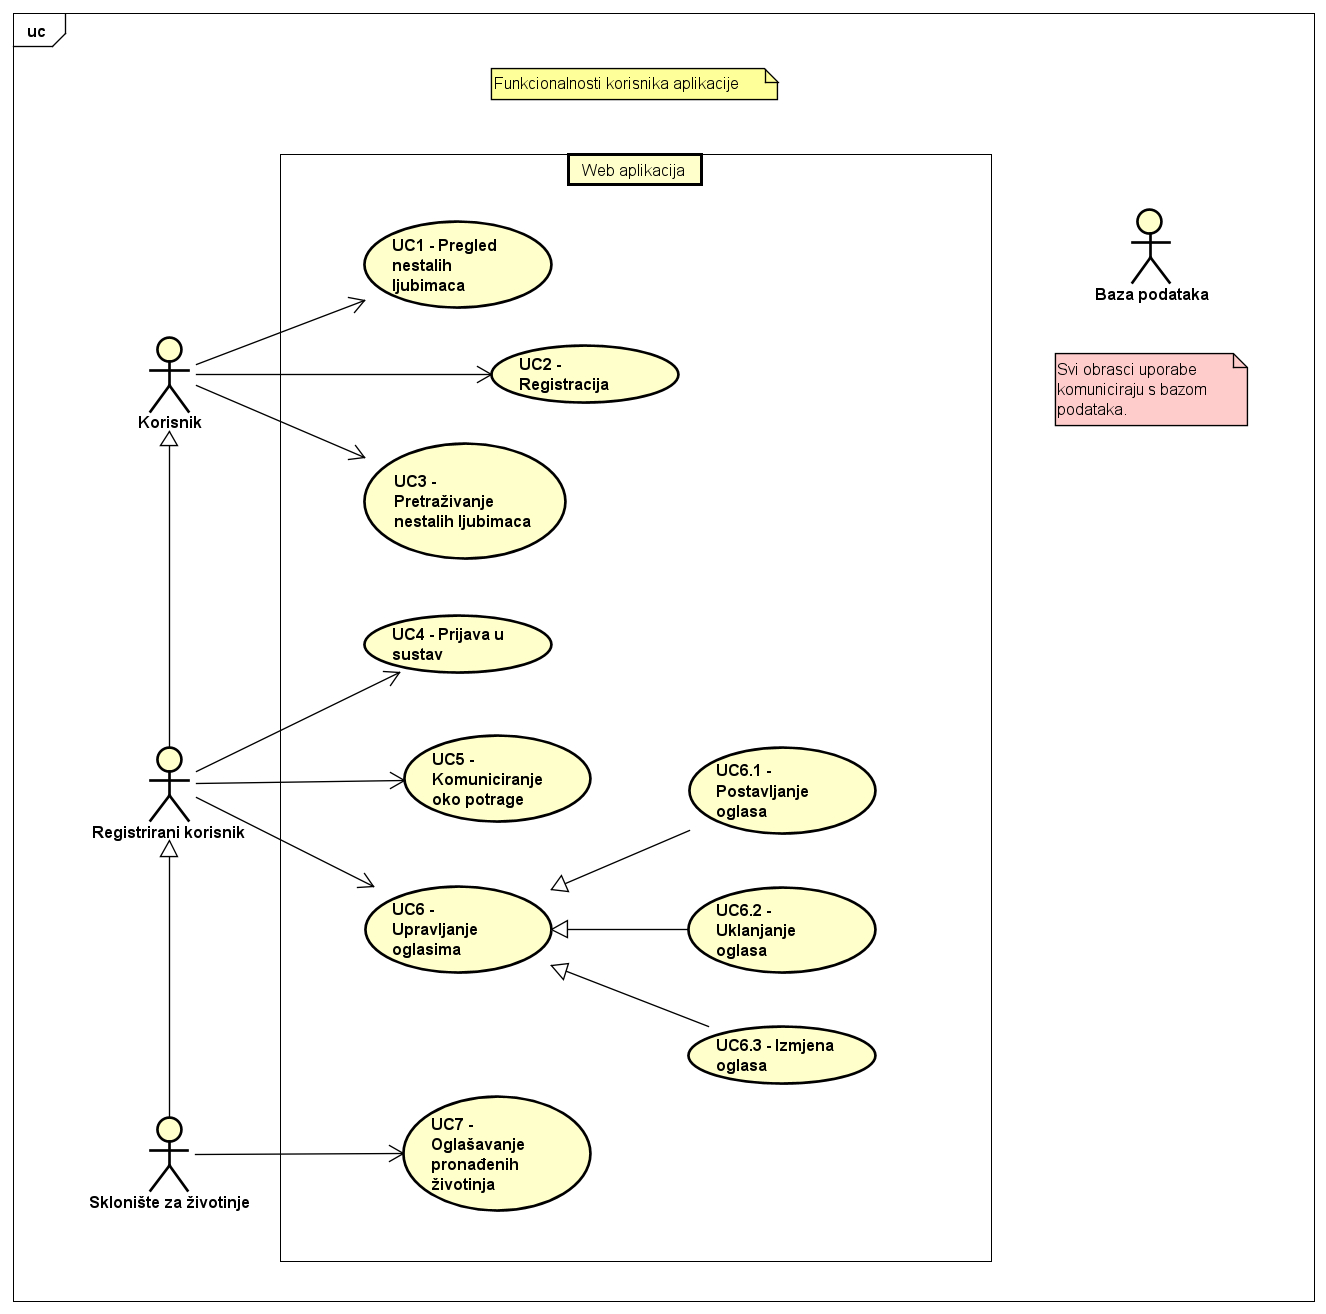
\includegraphics[width=\textwidth]{slike/funkcionalnosti_korisnika.png}
						\caption{Dijagram obrasca uporabe, funkcionalnost korisnika}
					\end{figure}		
				
			\pagebreak
			\subsection{Sekvencijski dijagrami}
				
				\textbf{\textit{dio 1. revizije}}\\
				
				\textit{Nacrtati sekvencijske dijagrame koji modeliraju najvažnije dijelove sustava (max. 4 dijagrama). Ukoliko postoji nedoumica oko odabira, razjasniti s asistentom. Uz svaki dijagram napisati detaljni opis dijagrama.}
				\eject
	
		\section{Ostali zahtjevi}
		
			\textbf{\textit{dio 1. revizije}}\\
		 
			 \textit{Nefunkcionalni zahtjevi i zahtjevi domene primjene dopunjuju funkcionalne zahtjeve. Oni opisuju \textbf{kako se sustav treba ponašati} i koja \textbf{ograničenja} treba poštivati (performanse, korisničko iskustvo, pouzdanost, standardi kvalitete, sigurnost...). Primjeri takvih zahtjeva u Vašem projektu mogu biti: podržani jezici korisničkog sučelja, vrijeme odziva, najveći mogući podržani broj korisnika, podržane web/mobilne platforme, razina zaštite (protokoli komunikacije, kriptiranje...)... Svaki takav zahtjev potrebno je navesti u jednoj ili dvije rečenice.}
			 
			 
			 
	